%%% CAPITOLO 2
%%% STRATEGIE DI TRADING E BACKTESTING

\section{Strategie di trading e backtesting}

Il backtesting ci permette di valutare la performance di una strategia di trading utilizzando
indicatori euristici o tecnici e applicandoli a dati storici.

Grazie al backtesting possiamo simulare la strategia di trading utilizzando dati storici e quindi generare risultati
ed analizzare il rischio oltre ad il potenziale profitto prima di investire vero capitale.

Nel contesto di questo progetto, è stato creato un algoritmo di trading usando le bande di bollinger per il signaling.

\subsection{Strategia buy/sell mediante Bollinger's Bands}

Le bande di Bollinger sono un metodo statistico per derivare informazioni sul prezzo e volatilità di un asset
nel tempo.

Per ottenere le bande di Bollinger abbiamo bisogno di calcolare la media mobile e la deviazione standard della serie
temporale, utilizzando una finestra specifica (tipicamente 20 giorni). Successivamente dobbiamo importare la banda
superiore/inferiore a $K$ volte (tipicamente 2) la deviazione standard mobile sopra o sotto la media mobile.

Per la strategia di trading scelta è stata impostata come finestra 20 giorni e come fattore di deviazione $2$.

La strategia prevede si creare un segnale di \emph{buy} nel caso di crossover da parte del prezzo della banda inferiore,
per quanto riguarda invece il segnale \emph{sell} ci deve essere un crossover nella banda superiore.

Di seguito il codice per la impostazione dei signal:

\begin{lstlisting}[language=Python]
    # Impostazione del buy signal
    self.buy_signal = bt.ind.CrossOver(self.datas[0],
                                       self.b_band.lines.bot)
    # Impostazione del sell signal
    self.sell_signal = bt.ind.CrossOver(self.datas[0],
                                        self.b_band.lines.top)
\end{lstlisting}

Se è presente già una posizione aperta non verranno aperte altre posizioni in caso di ulteriori cross-over, la posizione viene chiusa automaticamente
appena viene generato un segnale di sell.

L'algoritmo utilizzato non prevede short-selling, a causa di ciò per effettuare una operazione di sell deve essere presente una posizione aperta sul titolo, di seguito il codice che effettua l'ordine di acquisto o vendita:

\begin{lstlisting}[showstringspaces=false, language=Python]
    if not self.position:
        if self.buy_signal > 0:
            size = int(self.broker.getcash() / self.datas[0].open)
            self.log(f'BUY CREATED --- Size: {size},    \
                Cash: {self.broker.getcash():.2f},      \
                Open: {self.data_open[0]},              \
                Close: {self.data_close[0]}')
            self.buy(size=size)
    else:
        if self.sell_signal < 0:
            self.log(f'SELL CREATED --- Size: {self.position.size}')
            self.sell(size=self.position.size)
                 
\end{lstlisting}

\pagebreak

\subsection{Backtesting su titolo Meta (FB)}

Per effettuare il backtesting della strategia scelta, è stato preso in considerazione il titolo Meta (FB) nell'anno
2020, si può trovare il grafico a figura \ref{fig:fb_backtest}, come valore iniziale del portfolio sono stati impostati
$10000\$$ e per rendere i dati più reali è stata impostata anche una percentuale di commissione pari a $0.001\%$.

\begin{figure}[ht]
    \centering
    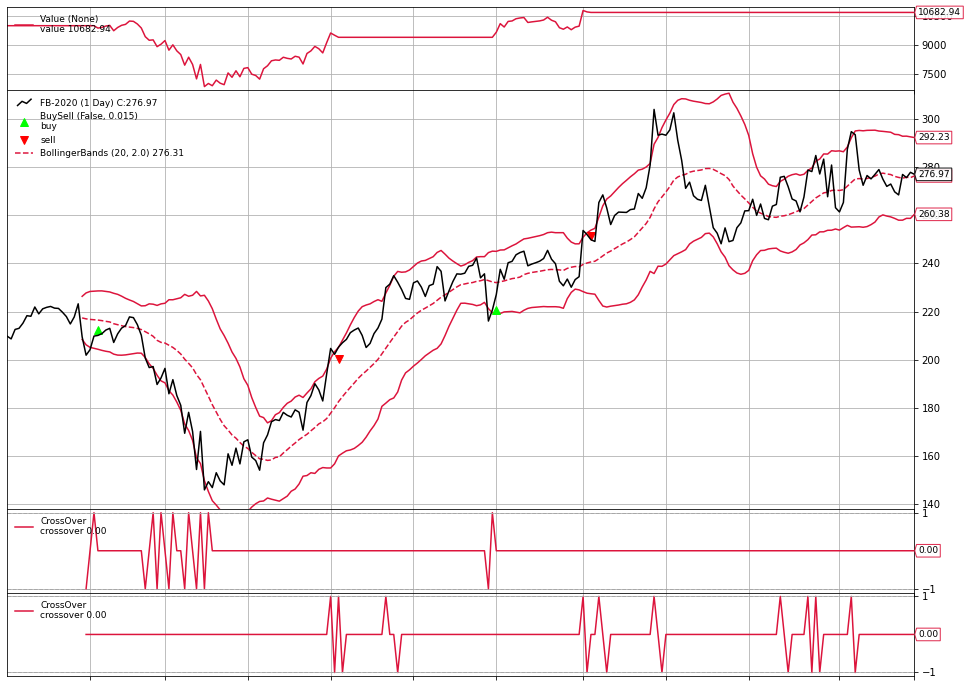
\includegraphics[width=1\textwidth]{fb_backtrack.png}
    \caption{Backtesting della strategia BB su FB}
    \label{fig:fb_backtest}
\end{figure}

\begin{figure}[ht]
    \centering
    \begin{minipage}{.5\textwidth}
        \centering
        \vspace{2.35cm}
        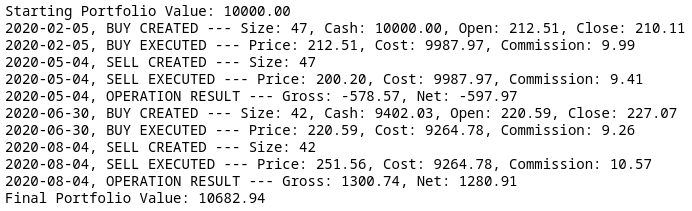
\includegraphics[width=.9\linewidth]{fb_backtrack_buy_sell.png}
        \captionof{figure}{backtrader log for FB}
        \label{fig:fb_backtr_log}
    \end{minipage}%
    \begin{minipage}{.5\textwidth}
        \centering
        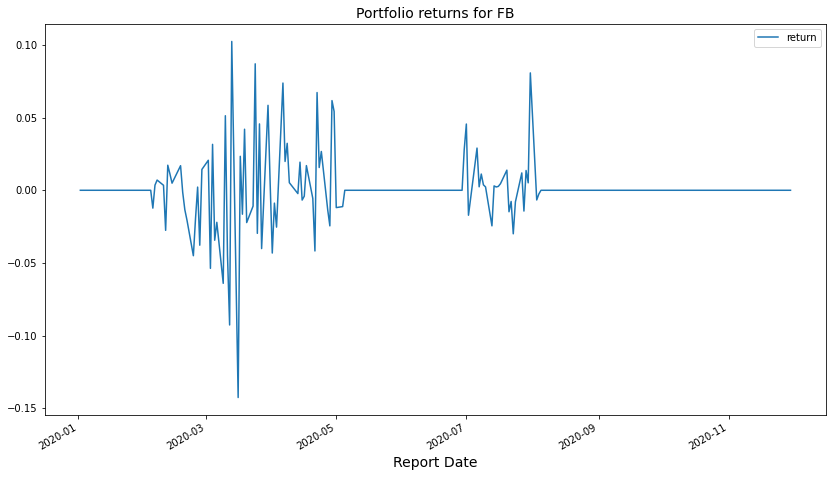
\includegraphics[width=1\linewidth]{fb_backtrack_ret.png}
        \captionof{figure}{Backtesting portfolio returns}
        \label{fig:fb_backtr_ret}
    \end{minipage}
\end{figure}

Dai log di \verb|backtrader| a figura \ref{fig:fb_backtr_log} si può vedere come la strategia è riuscita ad avere un profitto,
passando da $10000.00\$$ a $10682,94\$$ marcando un profitto di $682,94\$$ nel corso di un anno.\\
Analizzando i dati tecnici possiamo osservare un rendimento annuale/normalizzato pari al $7.47\%$.

Dal backtest è evidente come la strategia sia lontana dall'essere perfetta, dai due grafici presentati qui sopra si nota come nel
primo \emph{sell} ci sia stata una perdita sul valore del portfolio, al secondo \emph{sell} tuttavia la strategia è riuscita ad ottenere
un significativo rendimento che ha coperto la perdita del primo \emph{sell}.

\pagebreak